\section{\centering{"Query expansion using Language Models"}}

\begin{frame}{INTRODUCTION}
    Nowadays, searching the web for information appears to be one of the 
    simplest operations to perform. The difficulty perceived by the user in 
    formulating a query has been gradually reduced by techniques capable of 
    guiding his writing towards a correct generation of a query. These 
    techniques allow to improve the performance of information search 
    systems.
\end{frame}

\begin{frame}{GOAL}
    The purpose of this project is to be able to experiment with the use of 
    one of the most famous techniques, already present at the state of the 
    art, able to "assist" the user in formulating a correct query: {\bfseries Language 
    Modelling}. Query expansion can be done using this concept to return a 
    corpus of relevant documents. 
    \begin{minipage}{\linewidth}
        \centering
        \begin{minipage}{0.45\linewidth}
            \begin{figure}[h!]
                \centering
                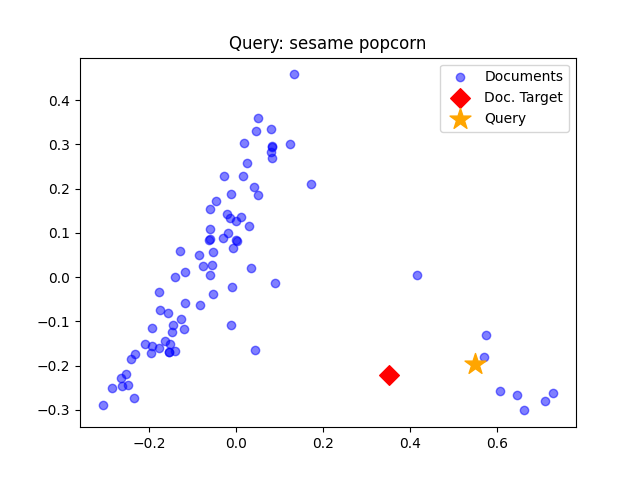
\includegraphics[width =\linewidth]{original_query.png}
                \centering
                \caption{Distance between initial query and target document in a PCA space.}
            \end{figure}
        \end{minipage}
        $\Rightarrow$
        \begin{minipage}{0.45\linewidth}
            \begin{figure}[h!]
                \centering
                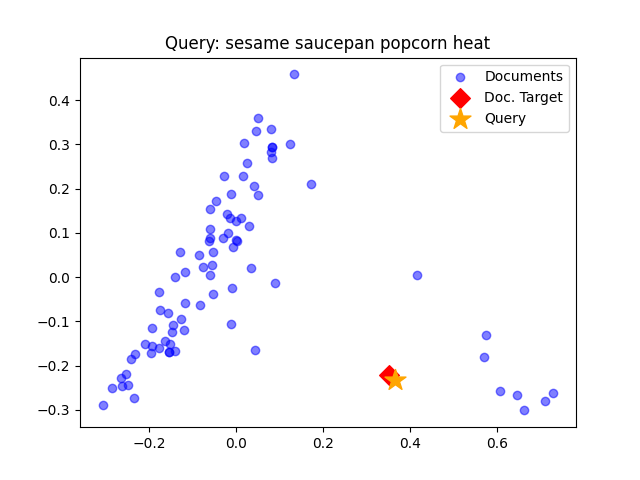
\includegraphics[width =\linewidth]{expanded_query.png}
                \centering
                \caption{Distance between the expanded query and the target document in a PCA space.}
            \end{figure}
        \end{minipage}
    \end{minipage}
\end{frame}

\begin{frame}{DATASET DESCRIPTION}
    \begin{minipage}{\linewidth}
        \centering
        \begin{minipage}{0.45\linewidth}
            The dataset used for the experiments is the famous \emph{Recipes1M+} \footnotemark, a collection 
            created by MIT, consisting of more than one million culinary recipes. Of 
            all these recipes, only a subset of 51235 documents of it was used due to their 
            informative content which best fits the purpose of this study. The information 
            about the line distributions for each recipe indicates that the instruction 
            field contains a higher number than the information contained in the ingredients 
            field.
        \end{minipage}
        \hspace{0.05\linewidth}
        \begin{minipage}{0.47\linewidth}
            \begin{figure}[h!]
                \centering
                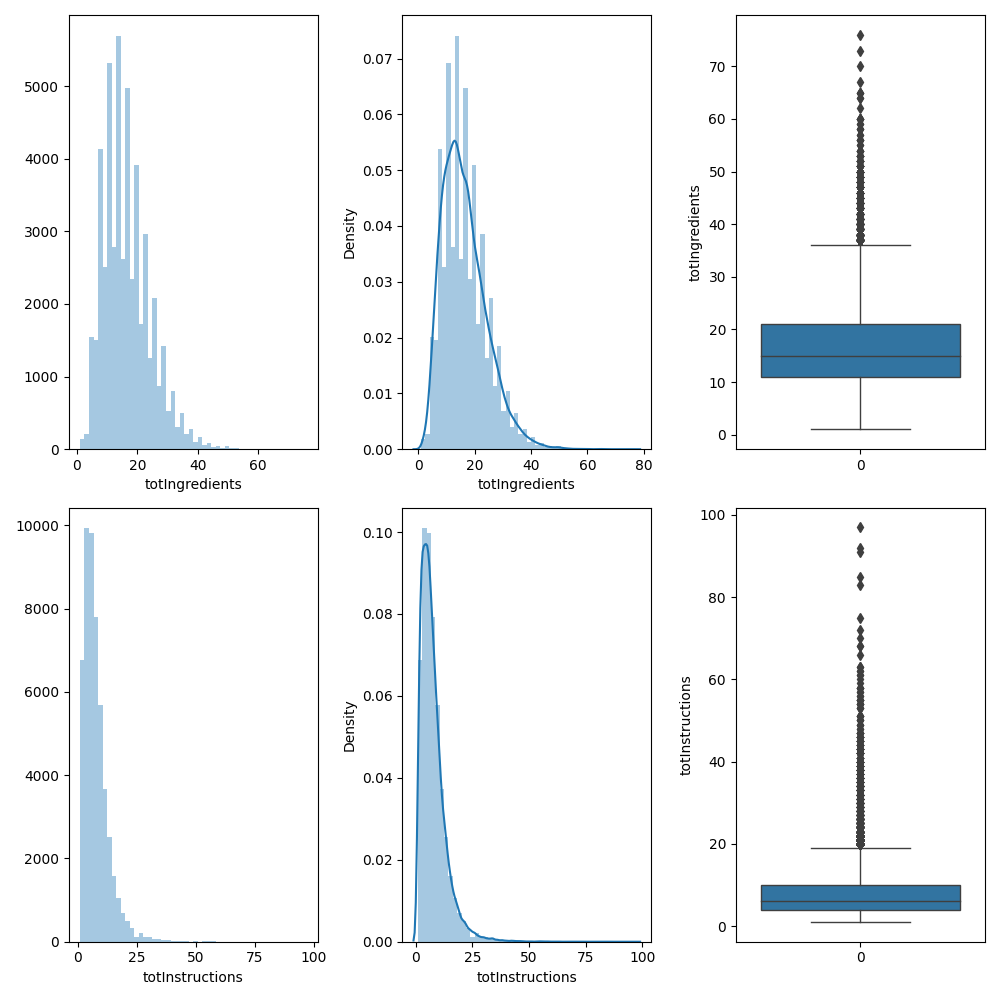
\includegraphics[width =\linewidth]{displot.png}
                \centering
                \caption{Distributions of lines per ingredients and instructions.}
                \label{distributions}
            \end{figure}
        \end{minipage}
    \end{minipage}
    \footnotetext{\tiny J.Marin, A.Biswas, F.Ofli, N.Hynes, A.Salvador, Y.Aytar, I.Weber and A.Torralba, "Recipe1M+: A Dataset for Learning Cross-Modal Embeddings for Cooking Recipes and Food Images", IEEE Trans. Pattern Anal. Mach. Intell., 2019}
\end{frame}

\begin{frame}{RANKING GENERATION}
    \renewcommand{\thefootnote}{\fnsymbol{footnote}}
    The first step is based on choosing a random query\footnotemark[1], which resembles the title of one of the existing recipes. Subsequently, thanks to the combination of the tf-idf method and the cosine similarity metric, it is possible to generate the first ranking of documents ordered according to relevance with the query. The threshold chosen, for the selection of the most relevant documents, will correspond to the weight assigned by the tf-idf to the target document.
    \begin{minipage}{\linewidth}
        \centering
        \begin{minipage}{0.45\linewidth}
            \begin{block}{\centering tf-idf}
                \centering \small $ TfIdf(q_t,d) = tf_{q_t,d} \log\frac{N}{df_{q_t}}$
            \end{block}
        \end{minipage}
        \hspace{0.05\linewidth}
        \begin{minipage}{0.45\linewidth}
            \begin{block}{\centering Cosine similarity}
                \centering \small $ cosine(q,d) = \frac{\sum_{i=1}^Nqd_i}{\sqrt{\sum_{i=1}^Nq^2}\sqrt{\sum_{i=1}^Nd_i^2}} $
            \end{block}
        \end{minipage}
    \end{minipage}
    \footnotetext[1]{\scriptsize \bfseries All documents (instructions of each recipe) and queries (recipe title) will undergo tokenization and normalization processes (removing stopwords / punctuation and applying lemmatization) before generating the ranking.}
\end{frame}

\begin{frame}{RANKING EVALUATION}
    The evaluation of the ranking of relevant documents was carried out considering 
    as the entity, of each single document, its category of belonging\footfullcite{16} 
    (dessert, salad, beverage, etc.). The search for each category takes place 
    in two methods, with two different libraries:
    \begin{itemize}
        \item \emph{Scrape Schema Recipe}
        \item \emph{USDA} (United States Department of Agricolture)
    \end{itemize}
    \begin{minipage}{\linewidth}
        \centering
        \begin{minipage}{0.50\linewidth}
            \begin{table}[]
                \centering
                \begin{adjustbox}{max width=\textwidth}
                \begin{tabular}{|c||c|c|c||c||c||}
                    \hline
                    \multirow{2}{*}{\bfseries{Queries}} & \multicolumn{3}{c||}{\bfseries{Scrape Schema Recipe}} & \multicolumn{1}{c||}{\bfseries{USDA}} & \multicolumn{1}{c||}{\bfseries{Mixed (Scrape+USDA)}} \\            & \bfseries{Overestimate} & \bfseries{Underestimate} & \bfseries{Discarded} & \bfseries{}  & \bfseries{}\\
                    \hline
                    \hline
                    \RN{1} & 0.7520 & 0.3734 & 0.5958 & 0.9817 & 0.9947\\
                    \hline
                    \RN{2} & 0.9309 & 0.6780 & 0.9054 & 1.0 & 1.0\\
                    \hline 
                    \RN{3} & 0.7458 & 0.2746 & 0.5411 & 0.9797 & 0.9982\\
                    \hline
                    \RN{4} & 0.8939 &  0.5320 & 0.8433 & 0.9612 & 0.9870\\
                    \hline
                    \RN{5} & 0.8335 & 0.5033 & 0.7544 & 0.9940 & 0.9940\\
                    \hline
                    \hline
                    Average & 0.8312 & 0.4722 & 0.7280 & 0.9833 &  \bfseries 0.99478 \\
                    \hline
                \end{tabular}
                \end{adjustbox}
                \caption{Average Precision on each query for each method.}
                \label{avgp}
                \centering
            \end{table}
        \end{minipage}
        \begin{minipage}{0.40\linewidth}
            \begin{figure}[htbp]
                \centering
                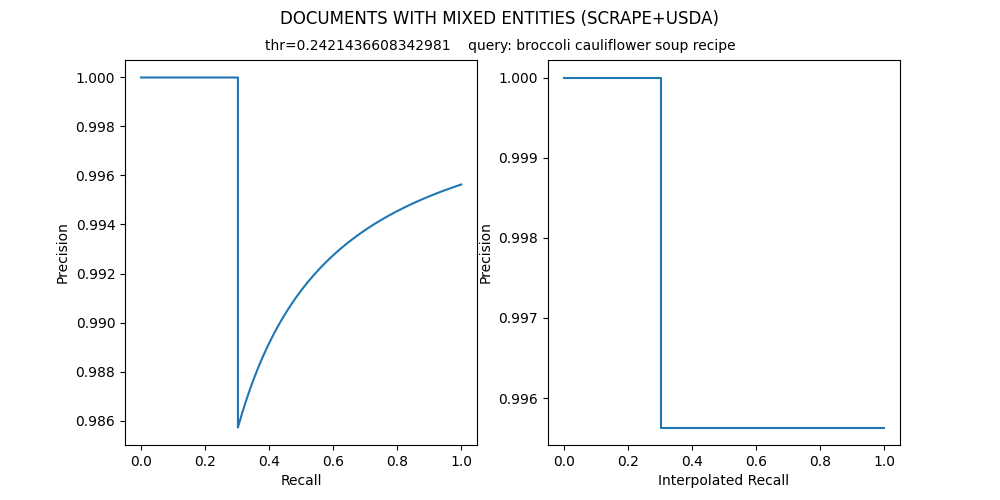
\includegraphics[width =\linewidth]{11 DOCUMENTS WITH MIXED ENTITIES (SCRAPE+USDA).png}
                \centering
                \caption{Performance in terms of Precion, Recall and Interpolated Recall.}
                \label{Performance mixed approach}
                \centering
            \end{figure}
        \end{minipage}
    \end{minipage}
\end{frame}

\begin{frame}{LANGUAGE MODELS}
    For each document, present in the ranking, a language 
    models will be constructed consisting of a sequence of \emph{bi-grams}, with an 
    initial \emph{skip-grams} equal to two, with the relative count of every 
    occurrence. Subsequently it will be possible to calculate the \emph{sentence 
    probability} (\ref{MLE}) between the query and each single language model.   
    \begin{block}{\centering Sentence probability (Bi-gram) and MLE}
        \begin{eqnarray}\label{MLE}
            P(q|d) & \approx & P(q|M_d) \nonumber \\
                   & \approx & \prod_i^n{P(w_i|w_{i-1})} \nonumber \\
                   & \approx & \prod_i^n\frac{count(w_i,w_{i-1})}{\sum_{j=1}^n count(w_j,w_{i-1})} \nonumber \\
                   & = & \prod_i^n\frac{count(w_i, w_{i-1})}{count(w_{i-1})}
        \end{eqnarray}
    \end{block}
\end{frame}

\begin{frame}{SMOOTHING METHODS}
    To avoid having a probability equal to zero, two smoothing techniques are calculated:
    \begin{minipage}{\linewidth}
        \centering
        \begin{minipage}{0.45\linewidth}
            \begin{block}{\centering Laplace Smoothing}
                \centering\small $ P(w_i|w_{i-1}) = \frac{count(w_{i-1})+1}{count(w_{i-1})+|V|} $
            \end{block}
        \end{minipage}
        \hspace{0.05\linewidth}
        \begin{minipage}{0.45\linewidth}
            \begin{block}{\centering Linear Interpolation Smoothing (Bi-grams)}
                \centering \scriptsize $ P(w_i|w_{i-1}) = \lambda P(q|M_d) + (1-\lambda)P(q|M_c) $
            \end{block}
        \end{minipage}
    \end{minipage}
    \begin{minipage}{\linewidth}
        \centering
        \begin{minipage}{0.45\linewidth}
            where:
            \begin{itemize}
                \item $\sum_i \lambda_i = 1$
                \item $M_d$: LM of the single document;
                \item $M_c$: LM of the entire collection of documents;
                \item $|V|$: \# unique words within the corpus of documents.
            \end{itemize}
        \end{minipage}
        \hspace{0.05\linewidth}
        \begin{minipage}{0.45\linewidth}
            \begin{figure}[H]
                \centering
                
\includegraphics[width =0.11\linewidth]{vertical points.png}
                \centering
            \end{figure}
            \begin{block}{\centering Linear Interpolation Smoothing (Zero-grams)\footnotemark}
                \centering \small $ P(w_i) = \lambda \frac{1}{|V|} + (1-\lambda)P(w_i) $
            \end{block}
        \end{minipage}
    \end{minipage}
    \footnotetext{\tiny A.Gutnik, "Log-Linear Interpolation of Language Models", 2000}
\end{frame}

\begin{frame}[fragile]{CORE}
    \begin{minipage}{\linewidth}
        \centering
        \begin{minipage}{0.60\linewidth}
            \begin{algorithm}[H]
                \algsetup{linenosize=\tiny}
                \scriptsize
                \SetKwInOut{Input}{input}
                \SetKwInOut{Output}{output}
                \SetKwData{LMcoll}{LMcoll}
                \SetKwData{rankLpl}{rankLpl}
                \SetKwData{LMdocs}{LMdocs}
                \SetKwData{PerplexityLpl}{perplexityLpl}
                \SetKwData{rankLinInt}{rankLinInt}
                \SetKwData{Lamb1}{lamb1}
                \SetKwData{Lamb2}{lamb2}
                \SetKwData{Break}{break}
                \SetKwData{PerplexityInt}{perplexityInt}
                \SetKwFunction{ComputeLMdocs}{ComputeLMdocs}
                \SetKwFunction{ComputeLMcoll}{ComputeLMcoll}
                \SetKwFunction{LplSmoot}{LplSmoot}
                \SetKwFunction{Perplexity}{Perplexity}
                \SetKwFunction{LinInt}{LinInt}
                \Input{q}
                \Output{final\_ranking}
                \Parameter{LMtd}
                \BlankLine
                \For{$s \leftarrow 2$ \KwTo $10$}{
                    \LMdocs$\leftarrow$ \ComputeLMdocs{$s, query $}\;
                    \LMcoll$\leftarrow$ \ComputeLMcoll{$s, query $}\;
                    rankLpl $\leftarrow$ \LplSmoot($q,LMdocs$)\;
                    perplexityLpl $\leftarrow$ \PerplexityLpl($q, LMtd$)\;
                    lamb1, lamb2 $\leftarrow$ 0\;
                    \For{$i \leftarrow 0.1$ \KwTo $1.0$}{
                        rankLinInt $\leftarrow$ \LinInt($q, LMdocs, LMcoll$)\;
                        perplexityInt $\leftarrow$ \PerplexityInt($q, LMtd$)\;
                        lamb1 $\leftarrow$ 0.1 + i\;
                        lamb2 $\leftarrow$ 0.9 - i\;
                        \If{lamb2==0}{break\;}       
                    }
                }
                \vdots
                \emph{Search for the minimum index of the target document}\;
                final\_ranking $\leftarrow$ min(rankLpl[i],rankLinInt[i])\;
                \Return{final\_ranking}
            \caption{Best Ranking\label{IR}}
            \end{algorithm}
        \end{minipage}
        \hspace{0.01\linewidth}
        \begin{minipage}{0.37\linewidth}
            \scriptsize
            where:
            \begin{itemize}
                \item \emph{q}: query
                \item \emph{s}: skip-gram
                \item \emph{final\_ranking}: ranking containing the target document in the position closest to the first
                \item \emph{LMtd}: Language model of target document 
                \item \emph{LMdocs}: List of the language models of each document
                \item \emph{LMcoll}: language model of the entire collection of documents
                \item \emph{lamb1}: $\lambda_1$
                \item \emph{lamb2}: $\lambda_2$
            \end{itemize}
        \end{minipage}
    \end{minipage}    
\end{frame}

\begin{frame}{TERM-TERM MATRIX}
    As explained in \footfullcite{12}, two or more words are considered synonymous, or 
    semantically important, if their \emph{vectors}, represented in a multidimensional 
    space, have a high \emph{cosine similarity}. To find out, we need to build a 
    matrix of terms, called \emph{term-term matrix}, where the \emph{co-occurrences} 
    between the terms present in the relevant documents and in the query 
    will be reported. We can exploit the \emph{Language Model} of the entire corpus, of relevant documents, to derive co-occurrences.
    \begin{table}[h!]
        \centering
        \begin{adjustbox}{max width=10cm}
        \begin{tabular}{*{7}{|c}|}%%{|c|c|c|c|c|c|c|}
            \hline
            & variation & broccoli & cauliflower & toss & substitute & $\cdots$\\
            \hline
            variation & 0 & \bfseries{1} & 0 & 0 & 0 &$\cdots$\\
            broccoli & 0 & 0 & \bfseries{5} & 0 & 0 & $\cdots$\\
            cauliflower & 0 & 0 & 0 & \bfseries{1} & 0 & $\cdots$\\
            toss & 0 & 0 & 0 & 0 & \bfseries{1} &$\cdots$\\
            substitute & 0 & 0 & \bfseries{1} &0 & 0 &$\cdots$\\
            $\cdots$ & $\cdots$ & $\cdots$ & $\cdots$ & $\cdots$ & $\cdots$ & $\cdots$\\
            \hline
        \end{tabular}
        \end{adjustbox}
        \caption{Co-Occurrence of words in Term-Term Matrix.}
        \label{table accuracy}
    \end{table}
\end{frame}

\begin{frame}{POSITIVE POINTWISE MUTUAL INFORMATIONS (PPMI)}
    Pointwise Mutual Information (PMI) was used to evaluate the relationship between two words.
    \begin{block}{PMI}
        \small \emph{\say{PMI draws on the intuition that the best way to weigh the association between two words is to ask how much more the two words co-occur in our corpus than we would have a priori expected them to appear by chance.}\footnotemark[4]}
    \end{block}
    In this case, its \emph{"Positive"} version (PPMI) was used to be able to remove negative values.
    \begin{minipage}{\linewidth}
        \centering
        \begin{minipage}{0.40\linewidth}
            \begin{block}{\centering PMI}
                \centering \small $ PMI(x,y) = \log_2\frac{P(x,y)}{P(x)P(y)} $
            \end{block} 
        \end{minipage}
        \hspace{0.05\linewidth}
        \begin{minipage}{0.50\linewidth}
            \begin{block}{\centering PPMI}
                \centering \small $ PPMI(x,y) = \max(\log_2\frac{P(x,y)}{P(x)P(y)}, 0) $
            \end{block}
        \end{minipage}
    \end{minipage}
\end{frame}

\begin{frame}{SINGULAR VALUE DECOMPOSITION (SVD)}
    The term-term matrix presents two types of problems that affect the 
    performance and the calculation of cosine similarity: {\bfseries{high 
    dimensionality}} and {\bfseries{sparsity}}. In order to reduce the dimensionality, the 
    \emph{Singular Value Decomposition (SVD)} technique was applied.
    \begin{minipage}{\linewidth}
        \centering
        \begin{minipage}{0.20\linewidth}
            \begin{block}{}
                \centering $ A = USV^T $
            \end{block}
            \begin{block}{}
                \centering $ \mathcal{D} = U*S $
            \end{block}
            \begin{block}{}
                \centering $ \mathcal{T} = S*V^T $
            \end{block}
        \end{minipage}
        \hspace{0.05\linewidth}
        \begin{minipage}{0.60\linewidth}
            Where:
            \begin{itemize}
                \item \emph{A}: a $t\times d$ Term-Term Matrix decomposed into 3 sub-matrices.
                \item \emph{U}: a $t\times m$ matrix
                \item \emph{S}: a $m\times n$ matrix
                \item \emph{$V^T$}: a $m\times d$ matrix
                \item \emph{$\mathcal{D}$}: a $t\times m$ matrix containing all the terms of the relevant documents
                \item \emph{$\mathcal{T}$}: a $m\times d$ matrix containing the query terms useful for calculating the cosine similarity with the terms present in $\mathcal{D}$
            \end{itemize}
        \end{minipage}
    \end{minipage}
\end{frame}

\begin{frame}{QUERY EXPANSION}
    After calculating the cosine similarity between the word vectors of the 
    relevant documents and the word vectors of the query, a maximum of ten 
    most similar words are selected for each single word in the query. Starting 
    from this assumption, by making a combination between the pairs of 
    words ($q_t$, $d_n$), the maximum number of new queries that can be 
    generated is: 
    $$ \#Queries = \prod_i^q (\#sim\_words_i) $$
    Where \emph{q} represents the number of tokens of the query and \emph{$\#sim\_words_i$} 
    represents the number of tokens most similar to each single token \emph{i} of the 
    query. Obviously some checks are made (eg word repetition), which could invalidate the 
    generation of the query. \bfseries All new queries will be processed by the 
    algorithm (\emph{Core}) in order to determine the best ranking of relevant 
    documents, which has the target document in the first positions.
\end{frame}

\begin{frame}{PERPLEXITY}
    \begin{minipage}{\linewidth}
        \centering
        \begin{minipage}{0.35\linewidth}
            The perplexity is calculated 
            between the initial 
            query/new\_queries and the language 
            models of the target document.The peculiarity 
            highlighted by the 
            system is that as the 
            number of skip-grams increases, 
            as the lambda parameters 
            of Linear Interpolation 
            Smoothing vary, 
            the perplexity gradually 
            decreases.
        \end{minipage}
        \hspace{0.01\linewidth}
        \begin{minipage}{0.55\linewidth}
            \begin{figure}[H]
                \centering
                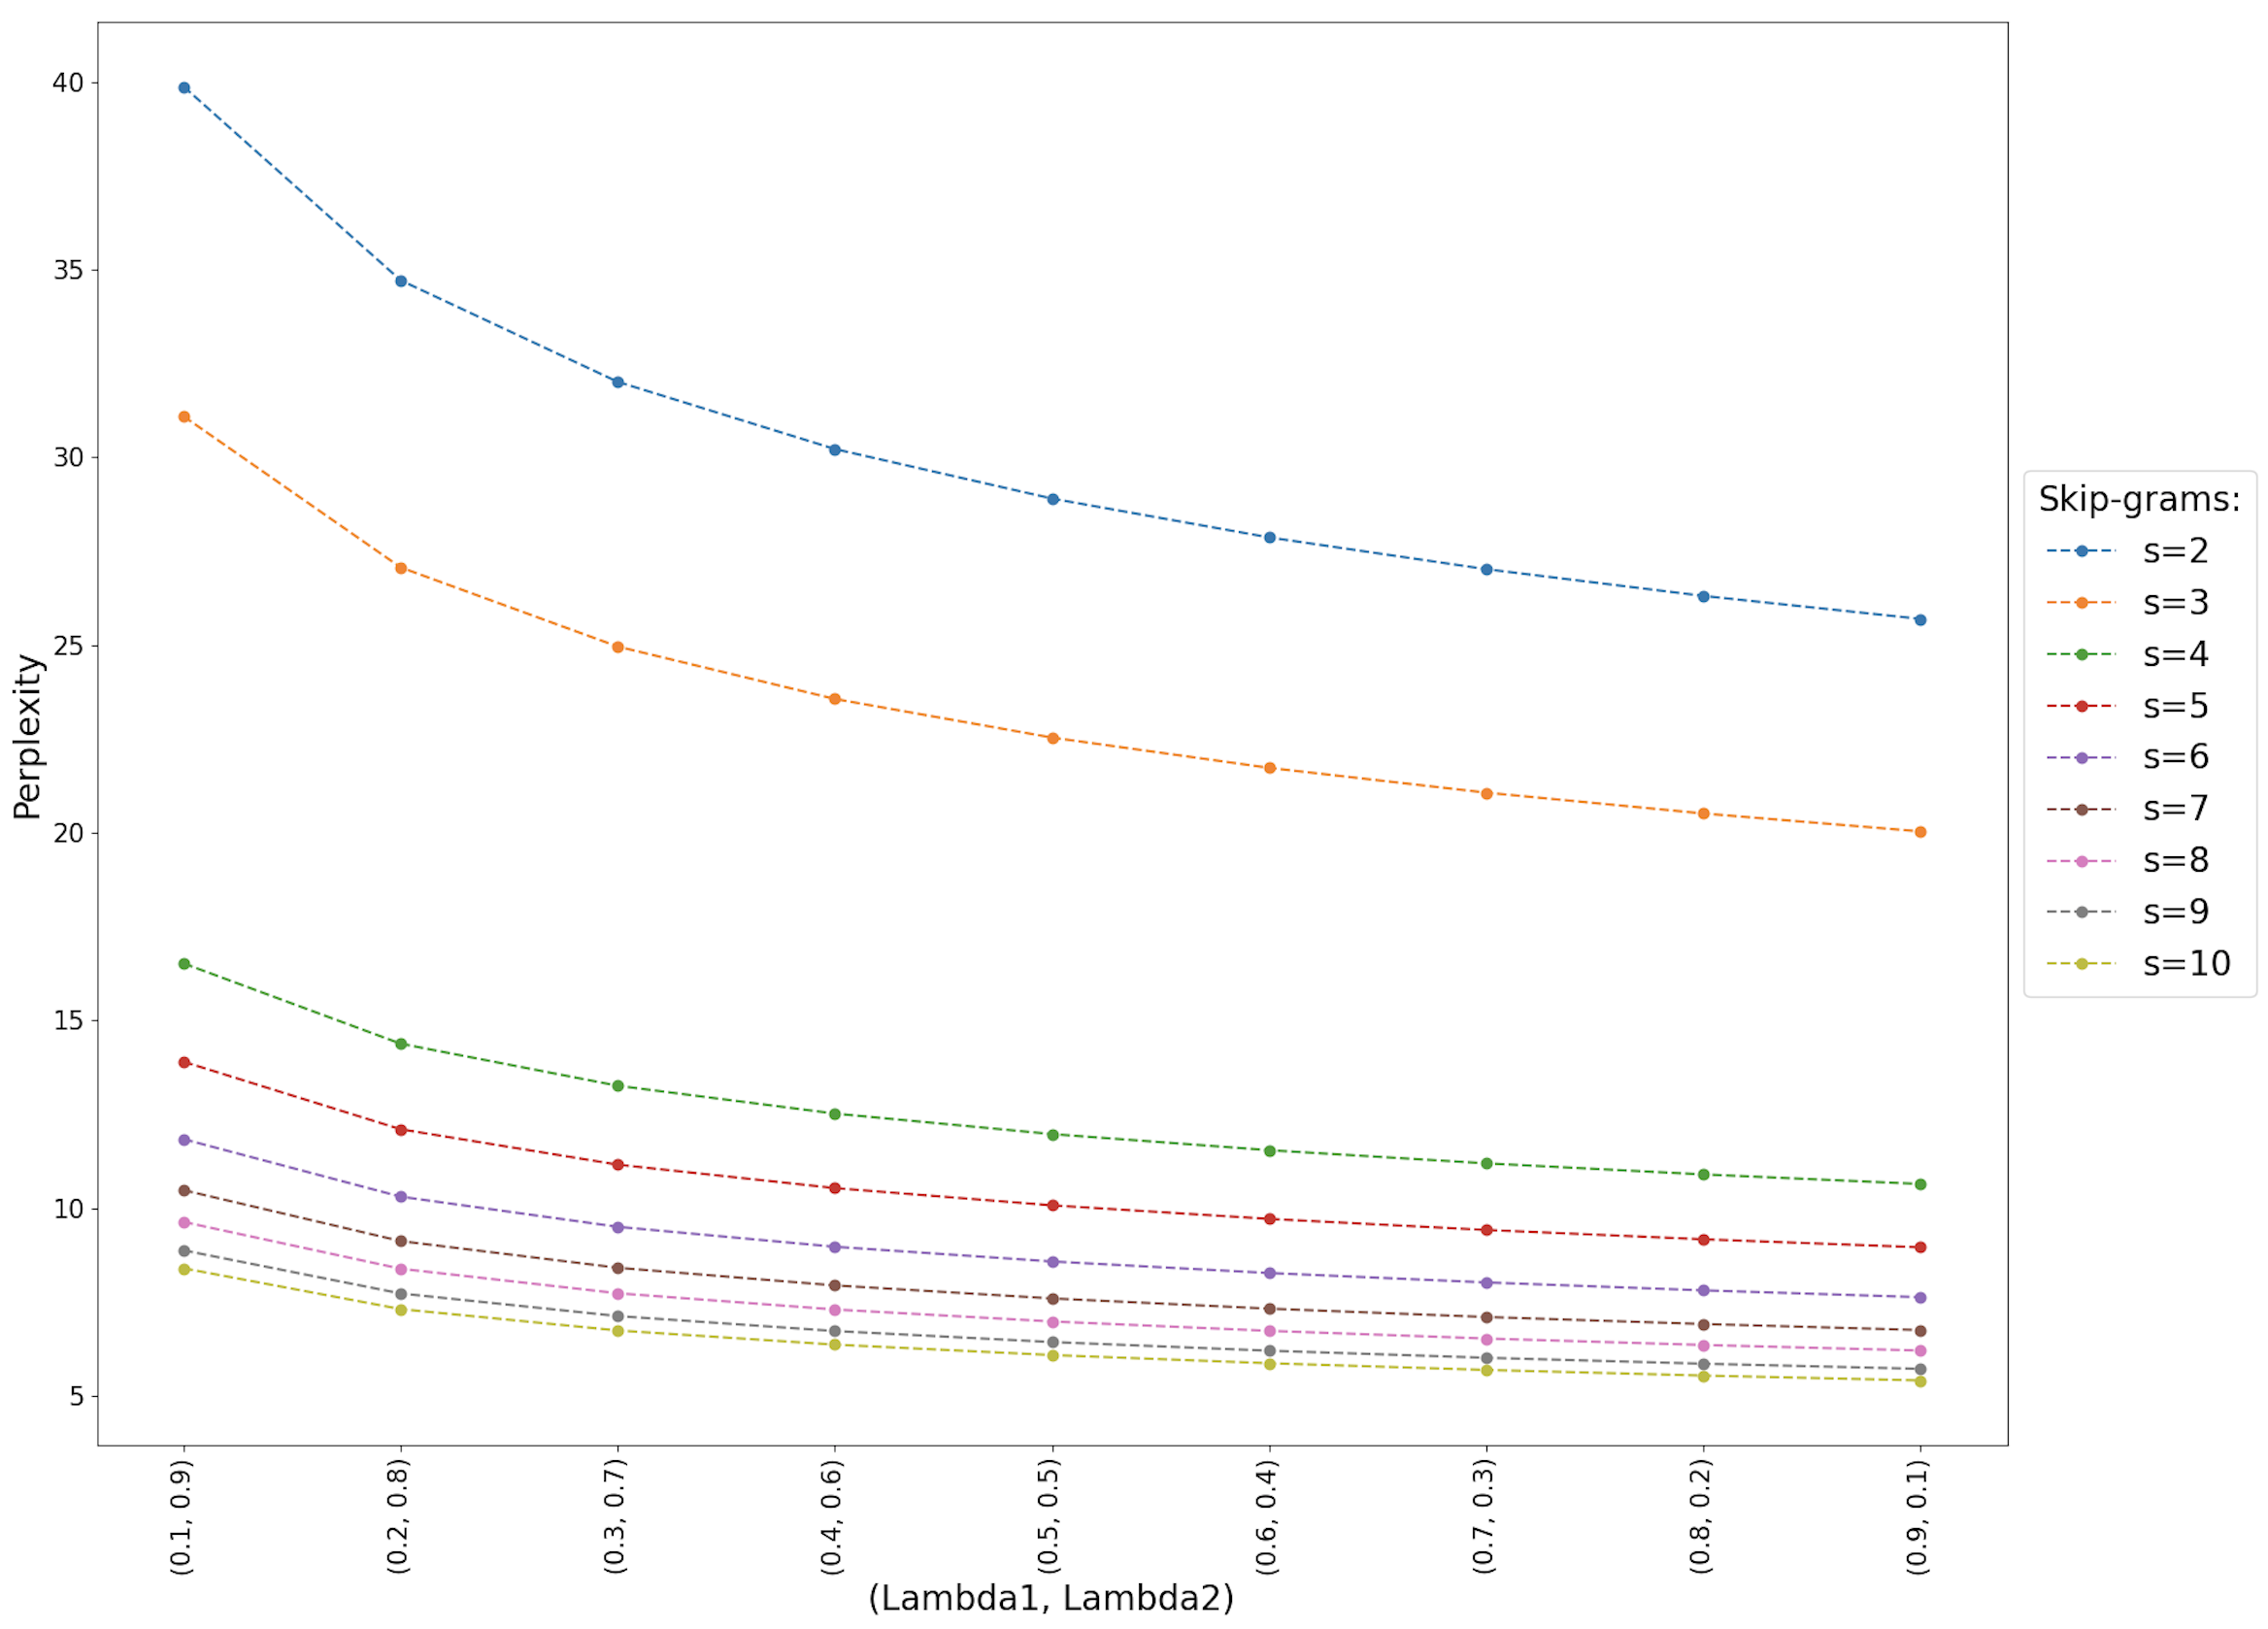
\includegraphics[width =\linewidth]{perplexity.png}
                \centering
                \caption{Variation of the perplexity value based on the change of the step \emph{s} and of the $\lambda_1$ and $\lambda_2$ values of interpolated smoothing.}
                \label{perplexity}
            \end{figure}
        \end{minipage}
    \end{minipage}
\end{frame}

\begin{frame}{SYSTEM EVALUATION WITH DIFFERENT PARSERS}
    To evaluate the performance of the system, four different parsers were 
    used: {\bfseries{Keras}}, {\bfseries{Nltk}}, {\bfseries{Spacy}} and {\bfseries{Gensim}}. The search results of the target
     document are compared with those obtained by the classic method tf-idf. 
     Each system has its own benefit but all of them manage, among the first 
     \emph{100} queries generated, to place the target document in the first position 
     of the ranking.
    \begin{table}[h!]
        \centering
        \begin{adjustbox}{max width=7cm}
        \begin{tabular}{|c||c|c||c|c||c|c||c|c||c|c||}
            \hline
            \multirow{2}{*}{\bfseries{Method}} & \multicolumn{2}{c||}{\bfseries{\RN{1}}} & \multicolumn{2}{c||}{\bfseries{\RN{2}}} & \multicolumn{2}{c||}{\bfseries{\RN{3}}} & \multicolumn{2}{c||}{\bfseries{\RN{4}}} & \multicolumn{2}{c||}{\bfseries{\RN{5}}}\\            & \bfseries{T} & \bfseries{P} & \bfseries{T} & \bfseries{P} & \bfseries{T} & \bfseries{P} & \bfseries{T} & \bfseries{P} & \bfseries{T} & \bfseries{P}\\
            \hline
            \hline
            Keras & \color{red}{228} & \color{green}{0} & \color{red}{623} & \color{green}{0} & \color{red}{82} & \color{green}{0} & \color{red}{126} & \color{green}{0} & \color{red}{51} & \color{green}{0}\\
            \hline
            Nltk & \color{red}{228} & \color{green}{0} & \color{red}{623} & \color{green}{0} & \color{red}{82} & \color{green}{0} & \color{red}{126} & \color{green}{0} & \color{red}{51} & \color{green}{0}\\
            \hline 
            Spacy & \color{red}{221} & \color{green}{0} & \color{red}{647} & \color{green}{0} & \color{red}{81} & \color{green}{0} & \color{red}{141} & \color{green}{0} & \color{red}{72} & \color{green}{0}\\
            \hline
            Gensim & \color{red}{240} &  \color{green}{0} & \color{red}{652} & \color{green}{37} & \color{red}{84} & \color{green}{0} & \color{red}{113} & \color{green}{0} & \color{red}{37} & \color{green}{0}\\
            \hline
        \end{tabular}
        \end{adjustbox}
        \caption{Target document position in the ranking of relevant documents. (T: \emph{tf-idf}, P:\emph{Proposed})}
        \label{Index}
    \end{table}
    \begin{table}[h!]
        \centering
        \begin{adjustbox}{max width=3.5cm}
        \begin{tabular}{|c|c|c|}
            \hline
            \bfseries{Method} & \bfseries{\#Queries} &\bfseries{Time}\\
            \hline
            \hline
            Keras & 14.900 &\bfseries{\emph{Low}}\\
            \hline
            Nltk & 14.900 &\bfseries{\emph{Low}}\\
            \hline
            Spacy & 19.010 &\emph{High}\\
            \hline
            Gensim & \bfseries{22.090} &\emph{Medium}\\
            \hline
        \end{tabular}
        \end{adjustbox}
        \caption{Performance in terms of number of queries (\#Queries) and computation time.}
        \label{performance}
    \end{table}
\end{frame}

\begin{frame}{PERPLEXITY AND DISTANCE EVALUATION WITH DIFFERENT PARSERS}
    Comparing all the systems, {\bfseries{Gensim}} manages to have, in most cases, a 
    \emph{low perplexity}, correlated to a \emph{low Euclidean distance}, between a new 
    generated query and the target document. These results make \emph{Gensim} 
    the best performing system.
    \begin{table}[h!]
        \centering
        \begin{adjustbox}{max width=8cm}
        \begin{tabular}{|c||c|c||c|c||c|c||c|c||}
            \hline
            \multirow{2}{*}{\bfseries{Queries}} & \multicolumn{2}{c||}{\bfseries{Keras}} & \multicolumn{2}{c||}{\bfseries{Nltk}} & \multicolumn{2}{c||}{\bfseries{Spacy}} & \multicolumn{2}{c||}{\bfseries{Gensim}}\\            & \bfseries{D} & \bfseries{P} & \bfseries{D} & \bfseries{P} & \bfseries{D} & \bfseries{P} & \bfseries{D} & \bfseries{P}\\
            \hline
            \hline
            \RN{1} & \color{red}{0.14} & \color{green}{16.41} & \color{red}{0.14} & {16.59} & \color{green}{0.12} & {34.89} & \color{red}{0.14} & \color{red}{90.17}\\
            \hline
            \RN{2} & {228} & {17.91} & \color{green}{0.11} & {22.37} & \color{red}{0.2} & \color{green}{11.57} & {0.15} & \color{red}{53.44}\\
            \hline 
            \RN{3} & {0.02} & \color{red}{5.41} & {0.02} & \color{red}{5.41} & \color{red}{0.07} & {5.15} & \color{green}{0.01} & \color{green}{5.03}\\
            \hline
            \RN{4}& {0.05} & {12.39} & {0.05} & \color{red}{12.45} & \color{red}{0.09} & {12.44} & \color{green}{0.01} & \color{green}{10.83}\\
            \hline
            \RN{5}& {0.31} & {23.04} & {0.31} & {23.22} & \color{red}{0.4} & \color{red}{42.25} & \color{green}{0.27} & \color{green}{10.36}\\
            \hline
            \RN{6}& {0.22} & {6.39} & {0.22} & \color{red}{6.39} & \color{red}{0.24} & {3.93} & \color{green}{0.21} & \color{green}{4.02}\\
            \hline
            \RN{7}& {0.12} & {1429.33} & {0.12} & \color{red}{1521.33} & \color{red}{0.24} & {6.03} & \color{green}{0.1} & \color{green}{3.43}\\
            \hline
            \RN{8}& {0.39} & {13.8} & {0.39} & \color{red}{13.81} & \color{red}{0.46} & {13.65} & \color{green}{0.27} & \color{green}{8.11}\\
            \hline
            \RN{9}& {0.56} &  \color{red}{5.3} & {0.56} & \color{red}{5.3} & \color{red}{0.6} & {4.7} & \color{green}{0.41} & \color{green}{3.9}\\
            \hline
            \RN{10}& {0} &  {4.29} & {0} & {4.29} & \color{red}{0.06} & \color{red}{5.12} & \color{green}{0} & \color{green}{4.28}\\
            \hline
        \end{tabular}
        \end{adjustbox}
        \caption{Euclidean Distance (D) between a query and the target document at a specific perplexity (P).}
        \label{DP}
    \end{table}
\end{frame}

\begin{frame}{CONCLUSIONS}
    Coming to the conclusions, it can be said that the generation of new 
    queries occurs correctly. However, there are some points that need to be 
    \underline{improved}, such as determining a method that sets an ad {\bfseries{\emph{hoc threshold}}} 
    useful for generating each ranking of relevant documents. Another 
    improvement concerns the reduction of the {\bfseries{sparsity}} of the term-term 
    matrix. This problem can be solved by applying techniques such as the 
    \emph{stochastic gradient descent}. As for \underline{future work}, however, it would be 
    interesting to develop a system of {\bfseries{hybrid parsers}}, fast and with low 
    perplexity. In addition to this development, it will be interesting to adopt 
    a new method of query expansion with terms present in a vocabulary 
    such as {\bfseries{Wordnet}}.
\end{frame}







